
\let\negmedspace\undefined
\let\negthickspace\undefined
\documentclass[journal,12pt,twocolumn]{IEEEtran}
\usepackage{cite}
\usepackage{amsmath,amssymb,amsfonts,amsthm}
\usepackage{algorithmic}
\usepackage{graphicx}
\usepackage{textcomp}
\usepackage{xcolor}
\usepackage{txfonts}
\usepackage{listings}
\usepackage{enumitem}
\usepackage{mathtools}
\usepackage{gensymb}
\usepackage[breaklinks=true]{hyperref}
\usepackage{tkz-euclide} % loads  TikZ and tkz-base
\usepackage{listings}

\begin{document}


\vspace{3cm}

\title{
%	\logo{
AI5030 - Software Assignment\\
Generating an audio playlist with random number generation%	}
}
\author{ Samuktha V. (AI23MTECH02004)

	\thanks{*The author is with the Department
		of Dept. of AI, Indian Institute of Technology, Hyderabad
		502285 India e-mail:  ai23mtech02004@iith.ac.in. All content in this manual is released under GNU GPL.  Free and open source.}
}

% make the title area
\maketitle

\newpage
\textbf{\emph{Aim:} To create an interactive GUI that enables playing the audio in random order}
\newline

\textbf{\emph{Given data :} Samples of 20 recorded videos  }
\newline
\newline
{\textbf{ \emph{Solution:}} A random number generator generates random numbers within a specified range.Here it has been utilised to generate an audio playlist in a random order. The numbers thus generated have a uniform distribution wherein each occurrence is equiprobable.}
{
This project ultimately plays audio files from a playlist randomly using a python code. In this we use the Moviepy for converting video files to audio, the os for importing the files, random for random selection of songs.
Initially the audio from the video has been extracted using Moviepy library in python.
The audio files thus extracted are saved in the same folder as the source code file and are later utilised for further processing.
}\\
 \textbf{Implementation :}\\
 This entire project uses python and these are the steps followed \\
 \begin{itemize}
     \item Extraction of audio: The program list of all the video files in a folder converted to audio files utilising the os library \\ 
  \item File selection and Randomization: After providing path of folder containing files, the program lists of all the audio files and shuffles them randomly \\
   \item Audio playback: The Moviepy library is used to load and play the audio files.This plays the songs in a sequence.
 
 \end{itemize}
 \textbf{Usage:} \\
To use this program these steps are to be followed: \\
\begin{itemize}
    
  \item The python is run to extract the audio files from the video playback in the folder "Videos" \\
 \item The extracted audio are saved in the same path as the code file and hence random generator code is to be run to fetch the audio files in a randomized fashion \\
 \item The interactive GUI enables easy navigation among various songs. 
\end{itemize}

\textbf{Conclusion:} 
The project's primary objective of creating play randomly in a chosen playlist with GUI functionality is successfully attained.
This programme encourages people to enjoy the song collection. This clearly demonstrates how Python was used to create a fun randomly played audio playlist.
\begin{figure}[h]
    \centering
    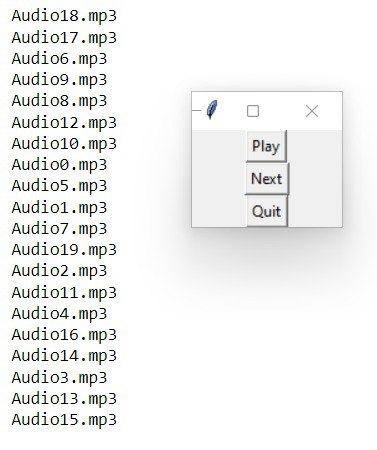
\includegraphics[scale=0.3]{gui.jpg}
    \caption{The list of the random playlist along with the GUI}
    \label{fig:my_label}
\end{figure}


\end{document}
